\clearpage
\section{Dashboards}
\label{sec:builder-feature-dashboards}

A dashboard is a page of numbers and charts that summarizes the work, such as the number of open requests or the average time to finish. You build it from widgets that take their data from a record type, form submissions or other sources, then publish it and place it in navigation. Each viewer sees the data their permissions allow, so a dashboard never goes around anyone's access.

\textbf{Path and who uses it:} “Builder” → “Core” → “Dashboards”. Built by those allowed to create dashboards, and viewed by those given access.

\begin{rcnote}[Example: Horizon]
Horizon builds a “Visit tracking” dashboard with a figure for pending requests, a chart of visits by branch and a calendar of their dates, which Sarah Al-Khatib reviews every week. The dashboard starts from ①.
\end{rcnote}

\begin{figure}[H]
\centering
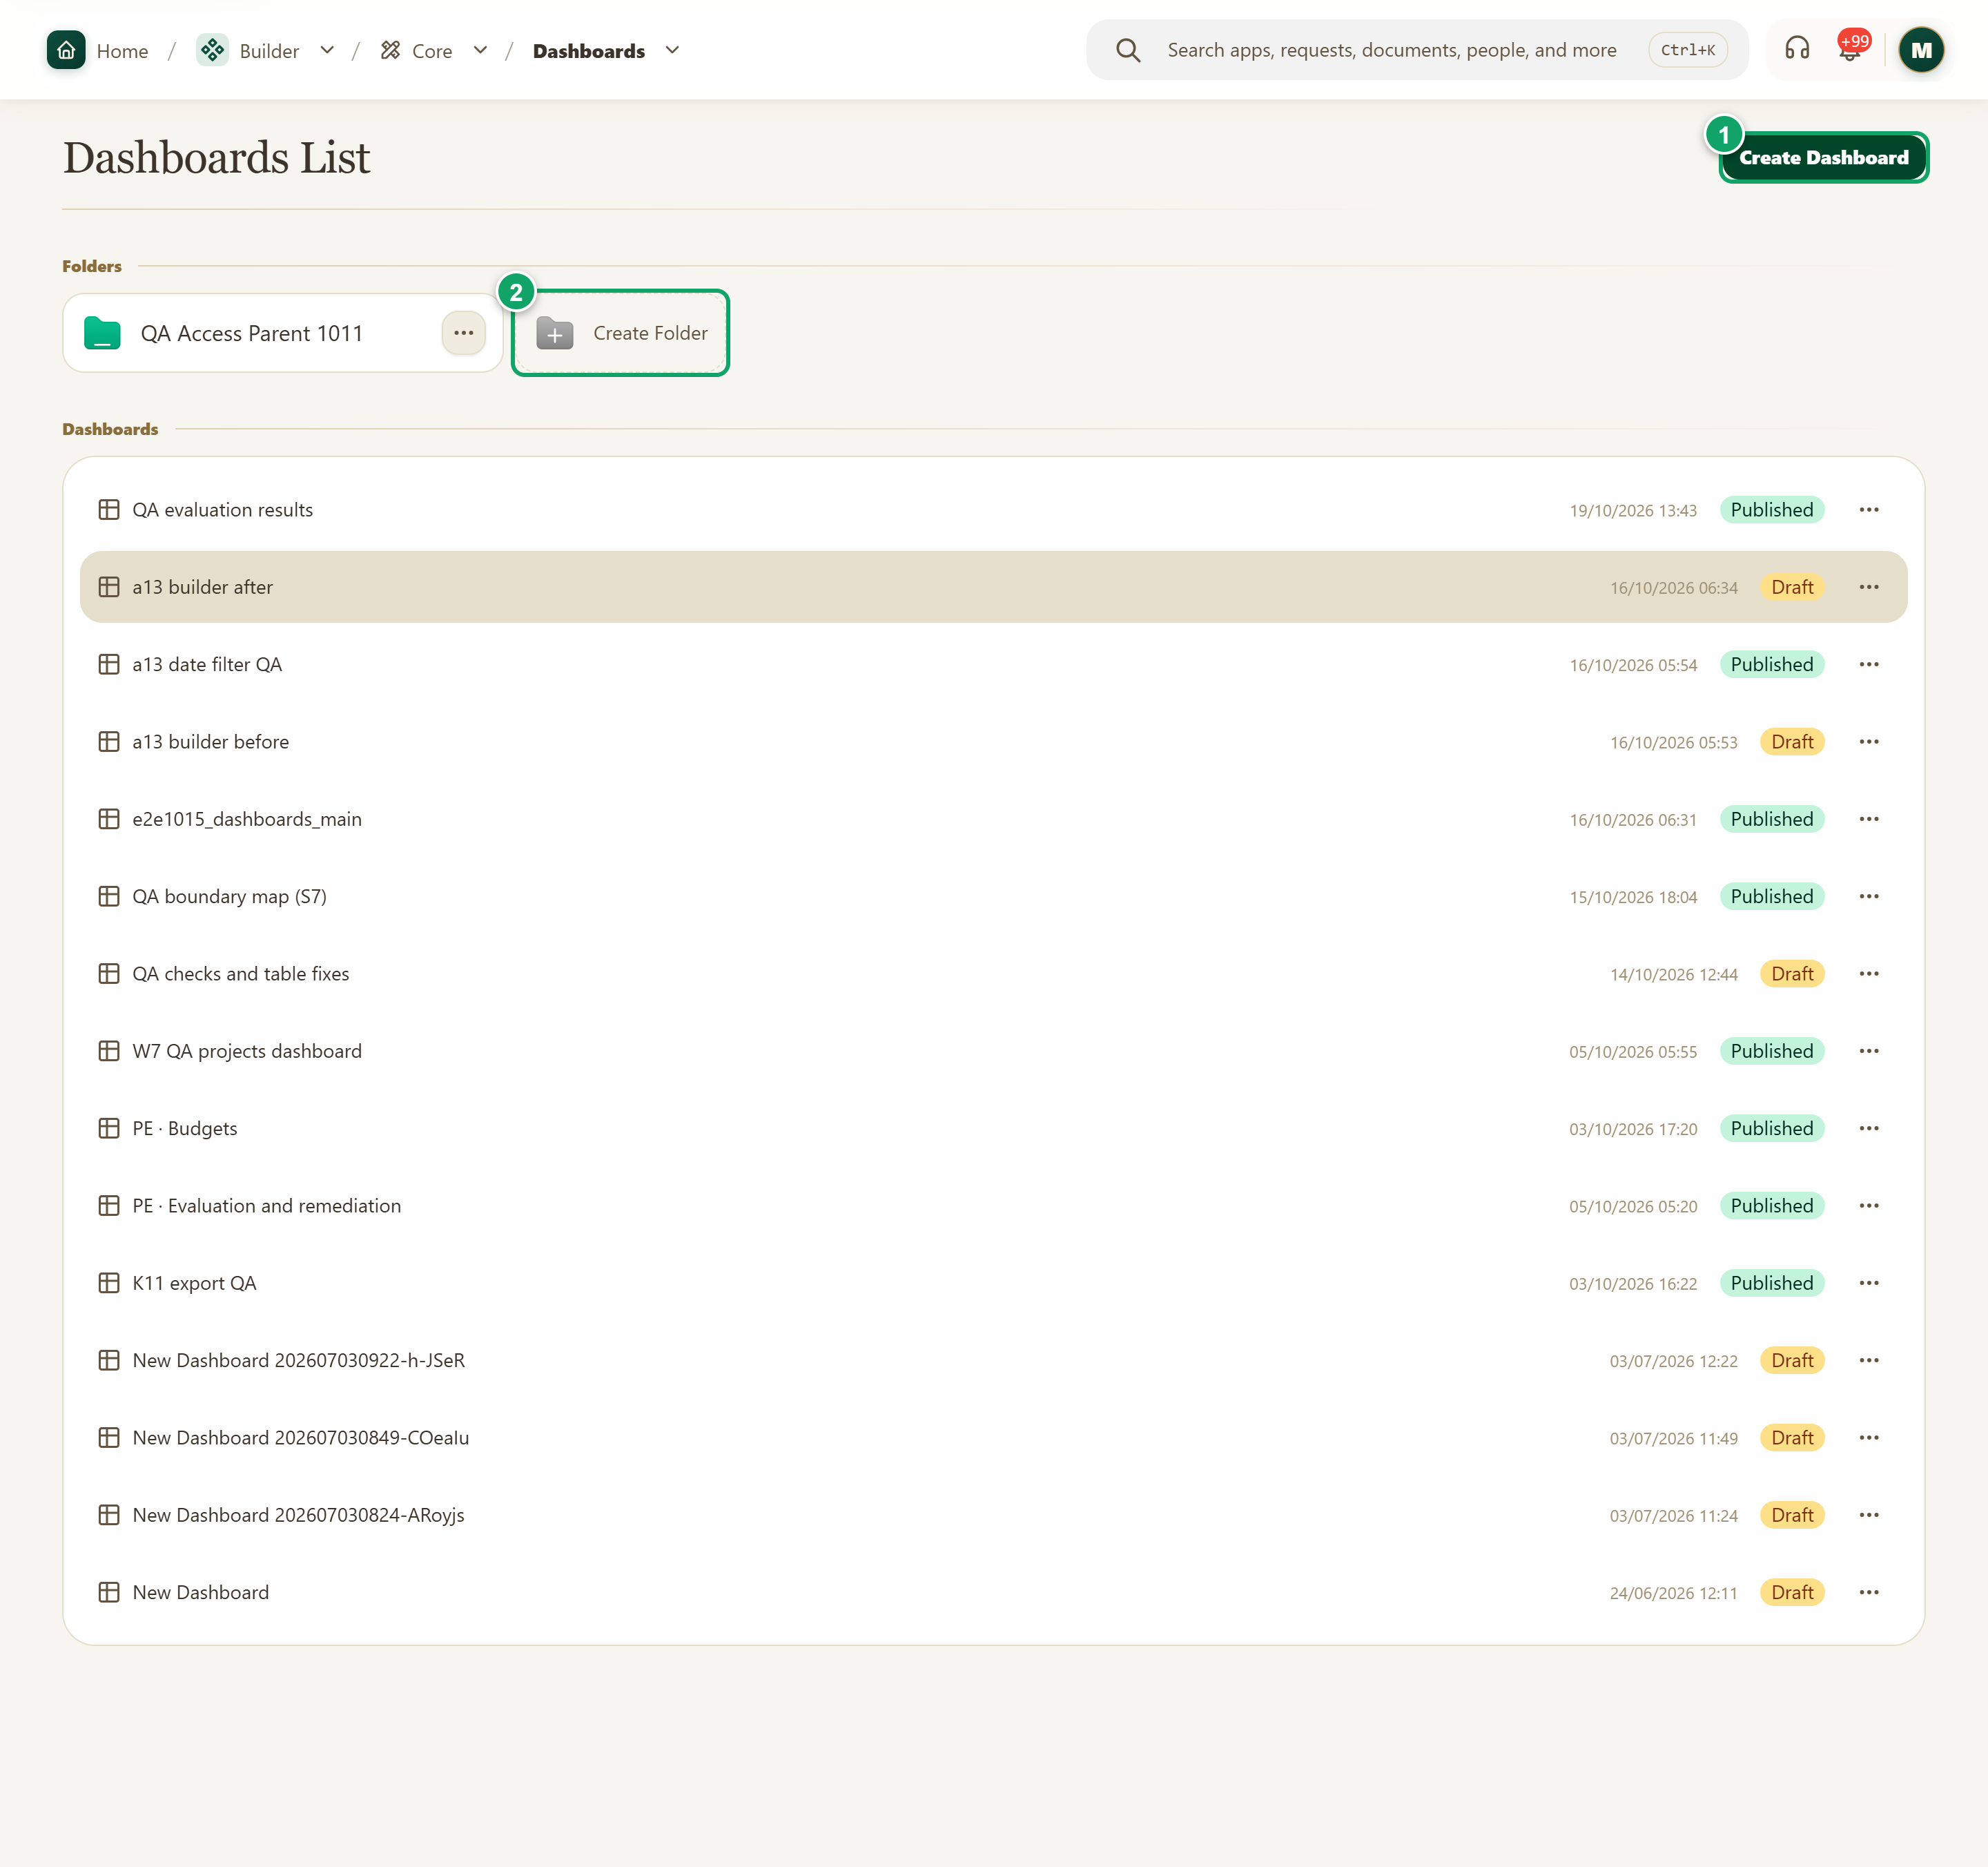
\includegraphics[width=0.95\linewidth,height=0.72\textheight,keepaspectratio]{figures/screens/ch06-dashboards-en.png}
\caption{The “Dashboards” page}
\label{fig:builder-dashboards-screen}
\shotnote{The page shows folders and dashboards with their status, here test dashboards. ① “Create Dashboard”: starts a new dashboard. ② “Create Folder”: organizes dashboards in folders.}
\end{figure}


\begin{table}[H]
\centering
\caption{What do you find here?}
\label{tab:builder-dashboards-data}
\begin{tabularx}{\linewidth}{R{3.6cm} Y}
\rcHeaderRow
\thh{Part} & \thh{Content and action}\\
Dashboards List & Dashboards and folders with their status, “Draft” or “Published”, and the buttons “Create Dashboard” and “Create Folder”.\\
Widgets & “Add Section”, then “Add Widget”: chart, figure, KPI, table, progress, calendar, map and more.\\
Data source & Entity, form submissions, SOP, manual data and others, with the data access level.\\
Filters & Let the viewer change the date range for the whole dashboard or for chosen sections or widgets.\\
Settings and access & Name, description, “Show in Navigation”, app and section, and “Manage access” to decide who views it.\\
Versions and publishing & “Publish” creates a new version that replaces the live one, and “Version history” lets you restore.\\
\end{tabularx}
\end{table}

\begin{figure}[H]
\centering
\begin{tikzpicture}[node distance=0.5cm]
\node[stepBox] (a) {Create Dashboard};
\node[stepBox,below=of a] (b) {Sections, widgets, sources};
\node[stepBox,below=of b] (c) {Preview and compare};
\node[stepBox,below=of c] (d) {Publish and show in navigation};
\draw[flowsTo] (a) -- (b);
\draw[flowsTo] (b) -- (c);
\draw[flowsTo] (c) -- (d);
\end{tikzpicture}
\rclegend
\caption{Building a dashboard}
\label{fig:builder-dashboards-flow}
\shotnote{The diagram puts the comparison with known records before publishing, because a wrong number on a dashboard leads to a wrong decision. If you know five requests are waiting for a decision, the widget must show five. The team does not see the dashboard in navigation before it is published.}
\end{figure}

\subsection{Steps and check}
\begin{enumerate}
\item Open “Dashboards” and press “Create Dashboard”, then write the name and a clear description.
\item Add a section, then a widget, choose its data source, fields and filters, and give it a title that says what it counts.
\item Press “Preview” and compare the numbers with records you know, then set where it appears in the settings and press “Publish”.
\end{enumerate}

\textbf{Check and recovery:} open the dashboard from navigation as a viewer; it should show the expected numbers. If the message “This dashboard isn't published yet” appears, publish it; if one user sees smaller numbers than another, it is because the dashboard shows what their permissions allow.

\clearpage
\section{Pages}
\label{sec:builder-feature-pages}

A page places a saved dashboard from the AI analytics workspace (\en{DB Genie}) inside an app section, so members see it as a menu item. It is the way to share a dashboard you made in “AI Dashboards” with the team.

\textbf{Path and who uses it:} “Builder” → “Core” → “Pages”. Available only to the organization owner and administrator.

\begin{rcnote}[Example: Horizon]
The system administrator makes an analysis of visit completion times in the AI workspace, then publishes it as a page in the “Visits” section of “Branch services” for Sarah Al-Khatib to see. The page starts from ①.
\end{rcnote}

\begin{figure}[H]
\centering
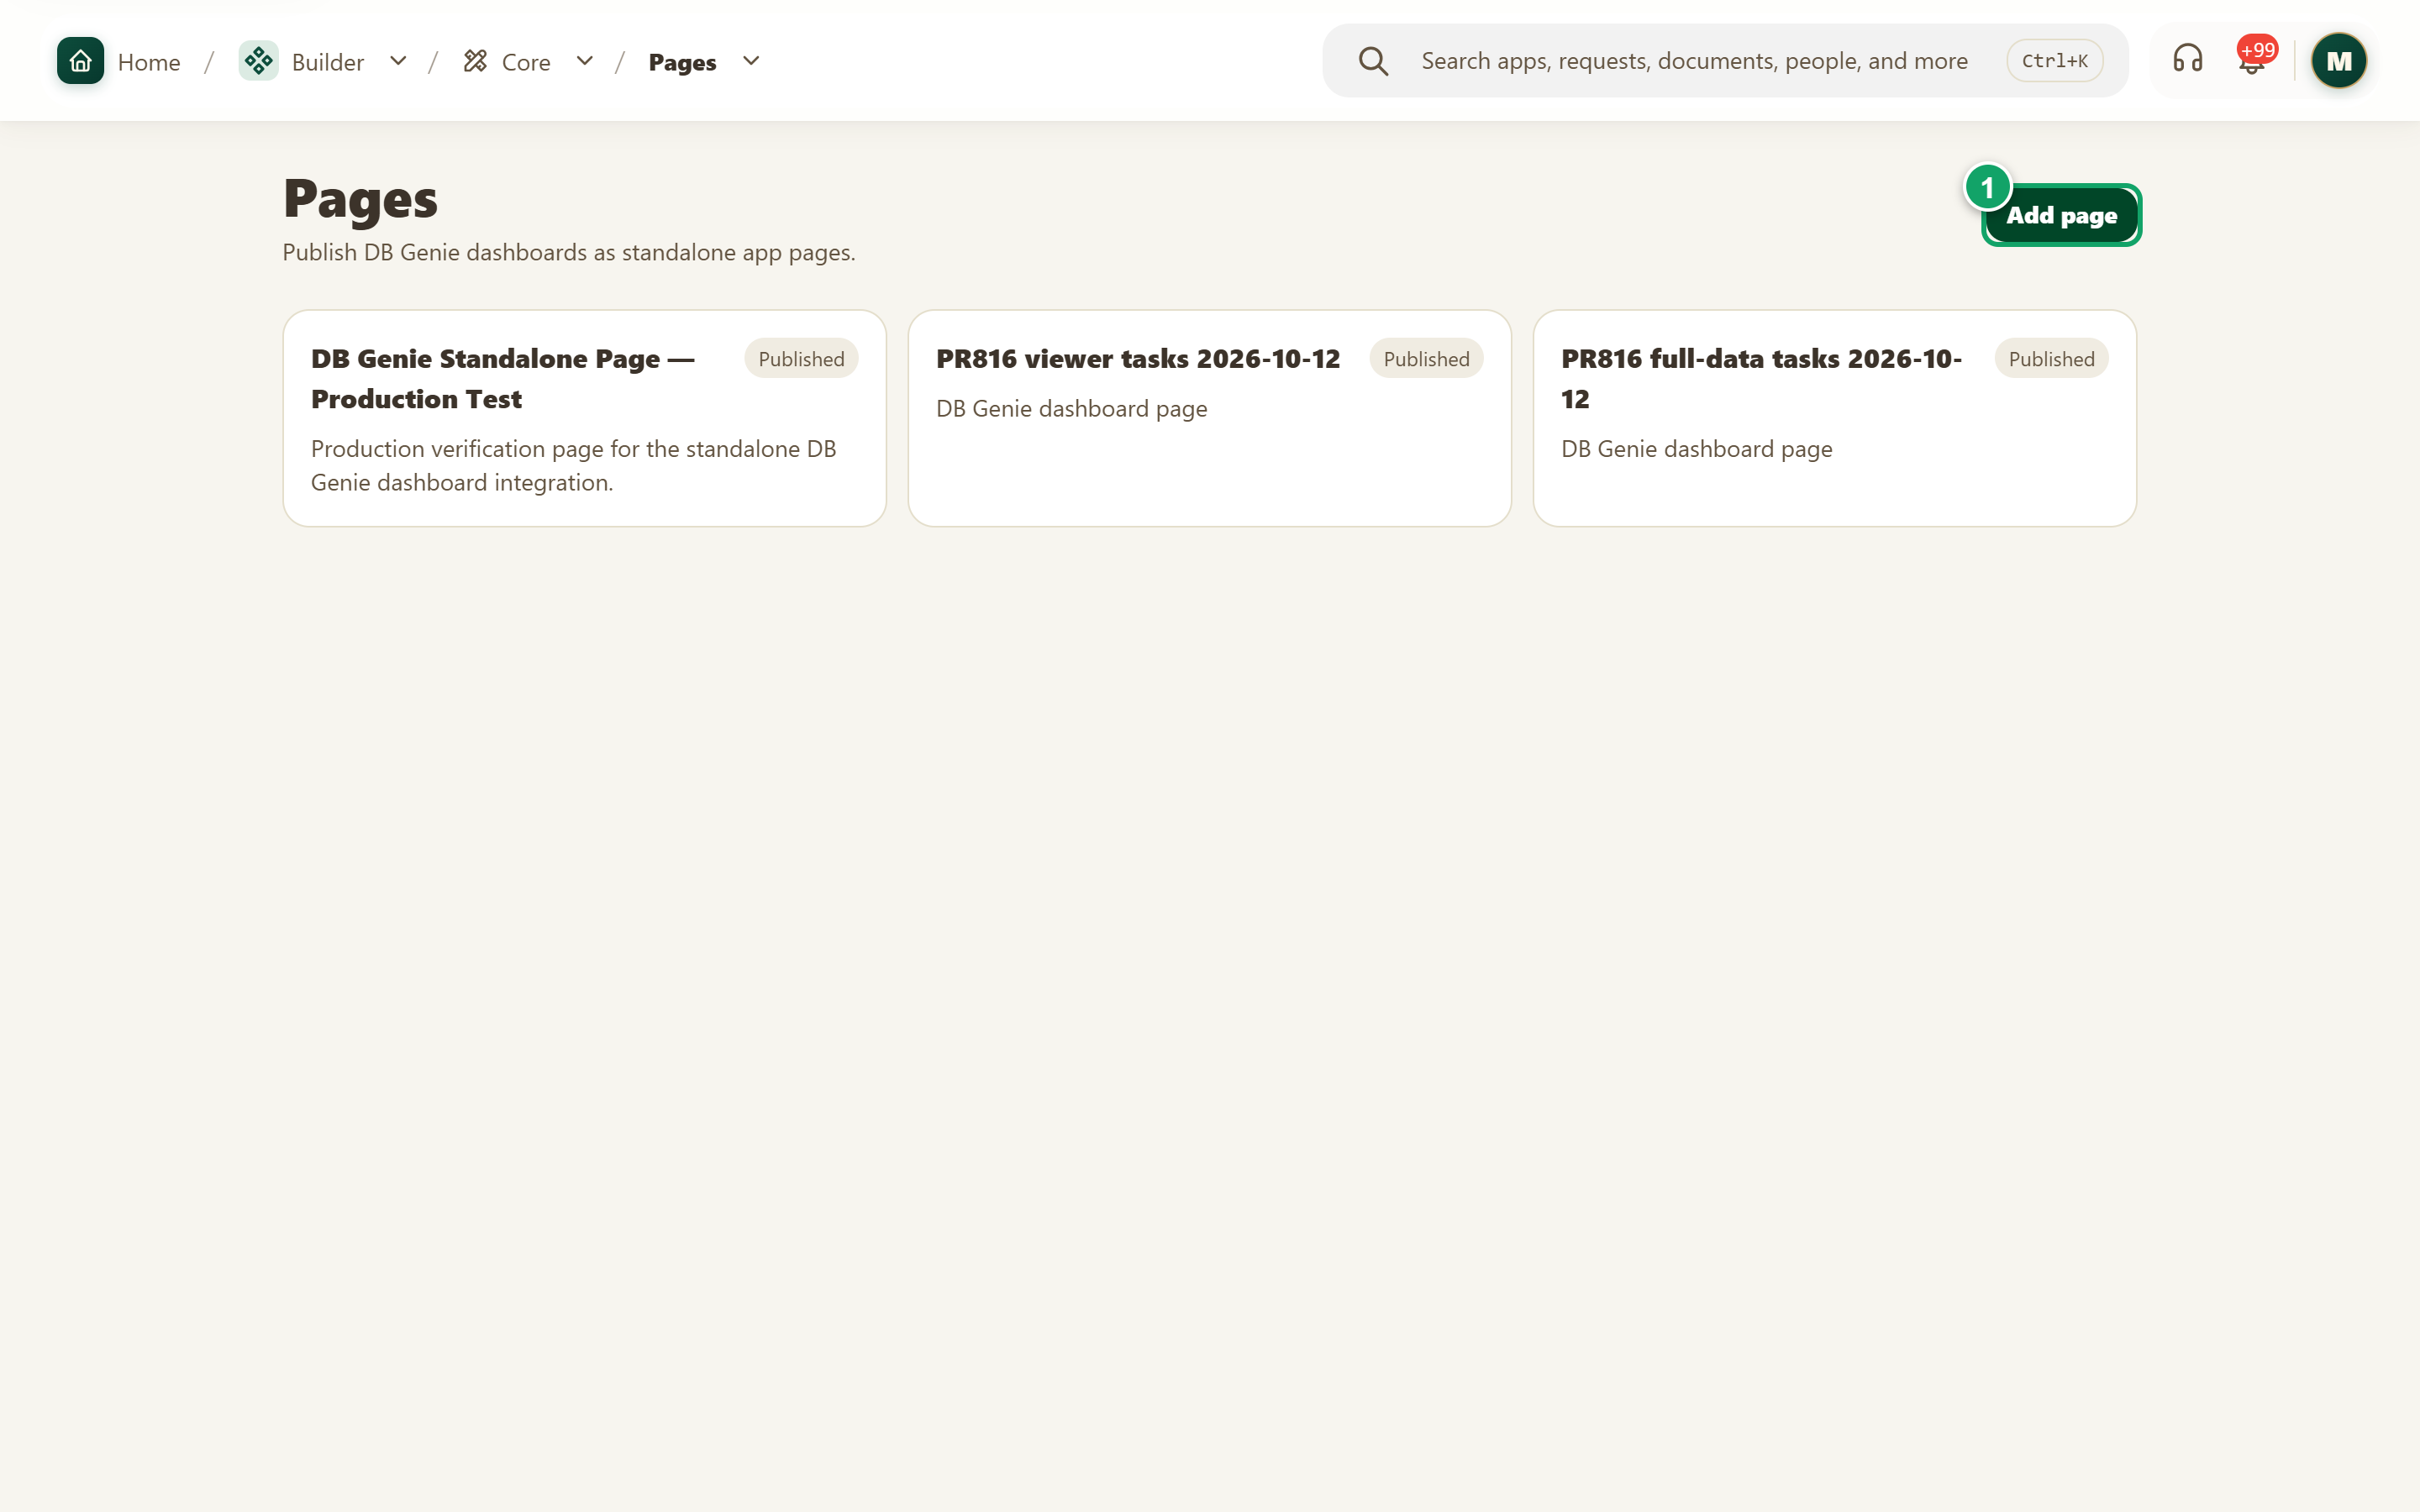
\includegraphics[width=0.95\linewidth,height=0.72\textheight,keepaspectratio]{figures/screens/ch06-pages-en.png}
\caption{The “Pages” page}
\label{fig:builder-pages-screen}
\shotnote{The page lists standalone pages published in apps, here test pages. ① “Add page”: starts a new page where you choose its dashboard, app and section.}
\end{figure}


\begin{table}[H]
\centering
\caption{The page's fields}
\label{tab:builder-pages-data}
\begin{tabularx}{\linewidth}{R{3.6cm} Y}
\rcHeaderRow
\thh{Field} & \thh{Meaning}\\
Title and Description & The page name as it appears in the menu, and a short description.\\
App and Section & Where the page appears in navigation.\\
DB Genie dashboard & A saved dashboard chosen with “Choose dashboard”.\\
Data shown & “With the viewer's permissions”, the safest choice, or organization data with guards, or all organization data without checking the viewer's scope.\\
Status & “Draft”, “Published” or “Archived”. The page appears in navigation only when published.\\
\end{tabularx}
\end{table}

\begin{figure}[H]
\centering
\begin{tikzpicture}[node distance=0.5cm]
\node[stepBox] (a) {Dashboard in the AI workspace};
\node[stepBox,below=of a] (b) {Add page, choose the dashboard};
\node[stepBox,below=of b] (c) {Status: Published};
\node[stepBox,below=of c] (d) {Grant roles the view right};
\draw[flowsTo] (a) -- (b);
\draw[flowsTo] (b) -- (c);
\draw[flowsTo] (c) -- (d);
\end{tikzpicture}
\rclegend
\caption{From a private dashboard to a team page}
\label{fig:builder-pages-flow}
\shotnote{The diagram shows that publishing the page is not enough for members to see it; each role also needs the right to view the page in the role settings. The original dashboard stays as it is, so deleting the page does not delete the dashboard.}
\end{figure}

\subsection{Steps and check}
\begin{enumerate}
\item Save the dashboard in “AI Dashboards” first.
\item Open “Pages” and press “Add page”, then write the title and choose the app, section and dashboard.
\item Choose “With the viewer's permissions” under “Data shown”, set the status to “Published”, then press “Save page”.
\item Give the right roles the right to view the page in the role settings.
\end{enumerate}

\textbf{Check and recovery:} the page should appear in the chosen section for those allowed to view it. If the message “Title, app, section, and dashboard are required.” appears, complete the four fields. If a member does not see it, check its status and their role's right.

\clearpage
\section{AI Dashboards}
\label{sec:builder-feature-ai-dashboards}

This page opens the AI analytics workspace (\en{DB Genie}), where you describe what you want to know and a dashboard is built for you from the organization's data. The workspace is private to you and uses only the data you can read. To share a dashboard with the team, publish it from the “Pages” page.

\textbf{Path and who uses it:} “Builder” → “Core” → “AI Dashboards”. Shown to those whose seat includes analytics, if they are an organization administrator or hold the right to view dashboards.

\begin{rcnote}[Example: Horizon]
Sarah Al-Khatib asks for a dashboard showing the number of visits per branch each month, and reviews the result in her private workspace before the system administrator decides to publish it as a team page. Sarah requests the dashboard inside workspace ①.
\end{rcnote}

\begin{figure}[H]
\centering
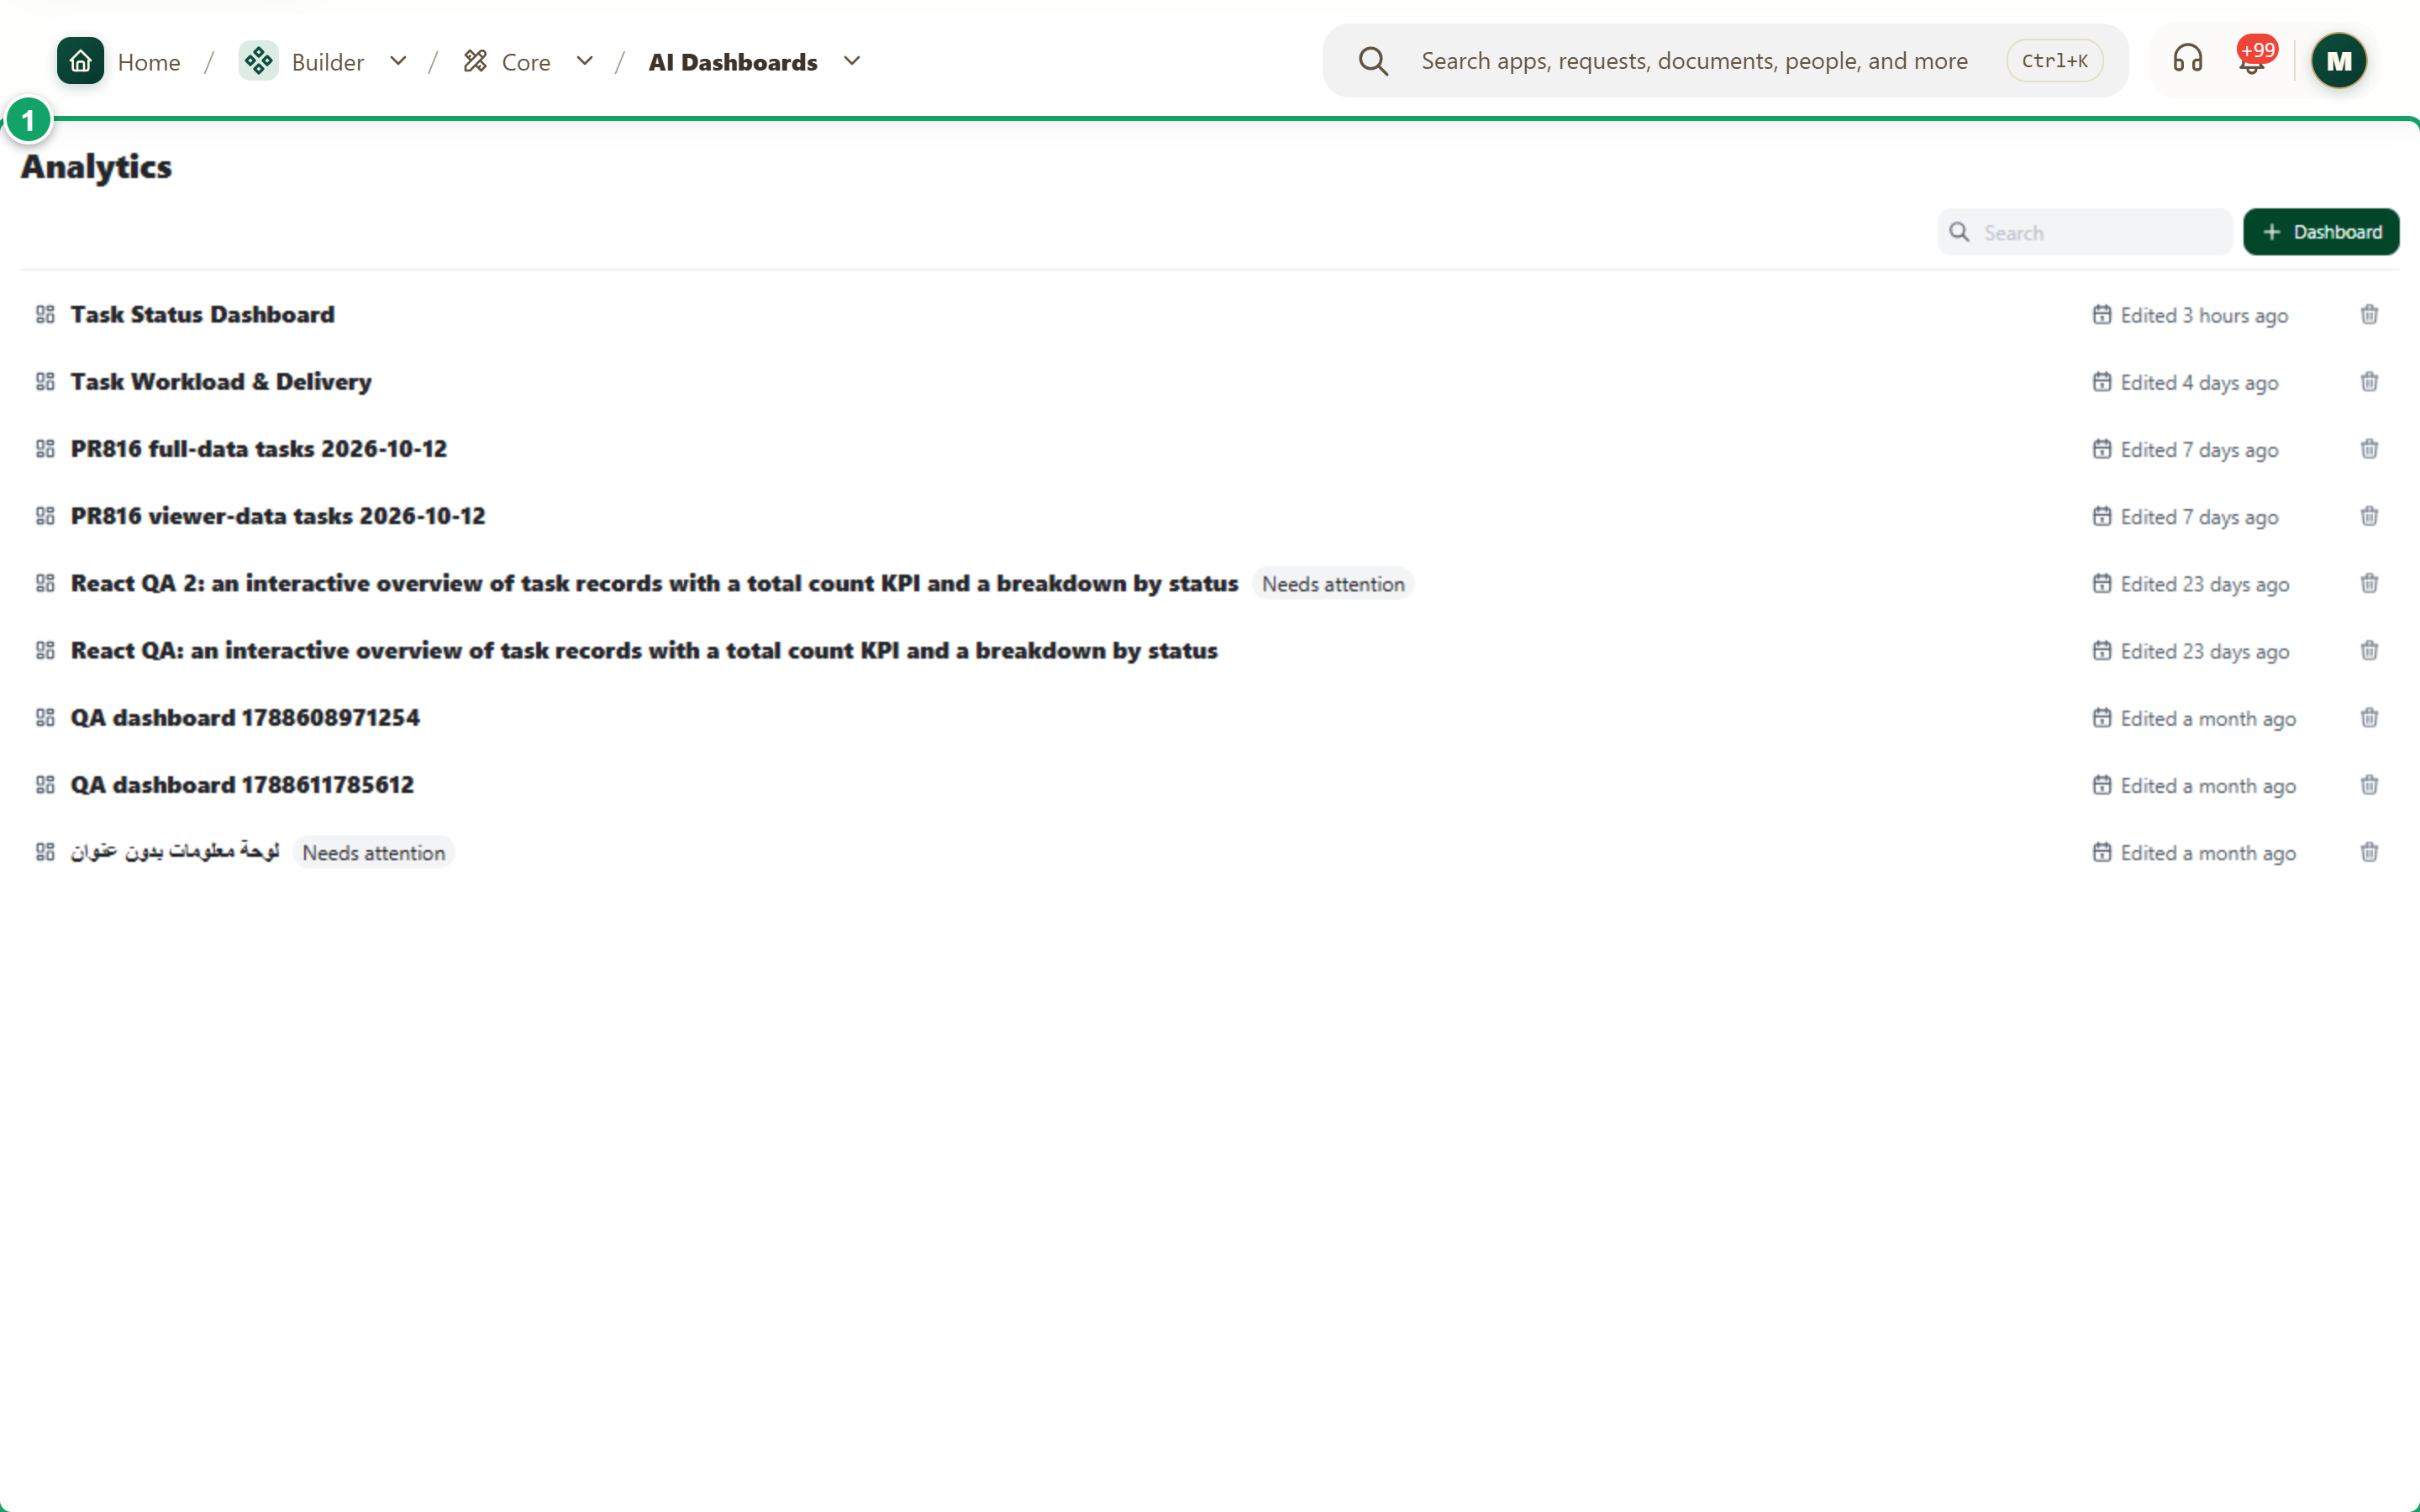
\includegraphics[width=0.95\linewidth,height=0.72\textheight,keepaspectratio]{figures/screens/ch06-ai-dashboards-en.png}
\caption{The “AI Dashboards” workspace}
\label{fig:builder-ai-dashboards-screen}
\shotnote{The analytics workspace opens inside KayanOS and shows the user’s own dashboards. The content here belongs to the test organization. ① The analytics workspace: where dashboards are created and reviewed, served by the embedded analytics system.}
\end{figure}


\begin{table}[H]
\centering
\caption{What should you know?}
\label{tab:builder-ai-dashboards-data}
\begin{tabularx}{\linewidth}{R{3.6cm} Y}
\rcHeaderRow
\thh{Aspect} & \thh{Meaning}\\
Private workspace & Dashboards here are yours alone and are computed only from data you are allowed to read.\\
Unavailable data & A message may say some data is unavailable because your access to certain record types is too broad to include.\\
Sharing & A dashboard is shared by publishing it as a page from “Pages”, not from this workspace.\\
\end{tabularx}
\end{table}

\begin{figure}[H]
\centering
\begin{tikzpicture}[node distance=0.5cm]
\node[stepBox] (a) {Describe what you want to know};
\node[stepBox,below=of a] (b) {Review the dashboard};
\node[stepBox,below=of b] (c) {Publish from Pages if needed};
\draw[flowsTo] (a) -- (b);
\draw[flowsTo] (b) -- (c);
\end{tikzpicture}
\rclegend
\caption{From a question to a shared dashboard}
\label{fig:builder-ai-dashboards-flow}
\shotnote{The diagram puts review before sharing, because an AI-generated dashboard may understand the question differently from what you meant. Compare its numbers with what you know, then share it through “Pages” only when you trust it.}
\end{figure}

\subsection{Steps and check}
\begin{enumerate}
\item Open “AI Dashboards” and wait for the analytics workspace to load.
\item Create a new dashboard and write clearly what you want to know, with the period and the important fields.
\item Review and save the dashboard, then publish it from “Pages” if the team should see it.
\end{enumerate}

\textbf{Check and recovery:} the workspace should open and show your dashboards. If “Could not open analytics” appears or the page sends you back home, your seat does not include analytics or you lack the right to view dashboards; ask the organization administrator.

\clearpage
\section{AI Reports}
\label{sec:builder-feature-ai-reports}

This page opens the same analytics workspace in chat mode: you ask in your own words about the organization's data, and the AI answers with a written report and numbers. It suits quick questions that do not need a permanent dashboard, such as “How many visits were cancelled this month, and why?”.

\textbf{Path and who uses it:} “Builder” → “Core” → “AI Reports”. It is shown under the same conditions as “AI Dashboards”.

\begin{rcnote}[Example: Horizon]
Sarah Al-Khatib asks which branches had visits delayed by more than a week, and gets a short report she uses in the monthly meeting. Sarah asks her question in area ①.
\end{rcnote}

\begin{figure}[H]
\centering
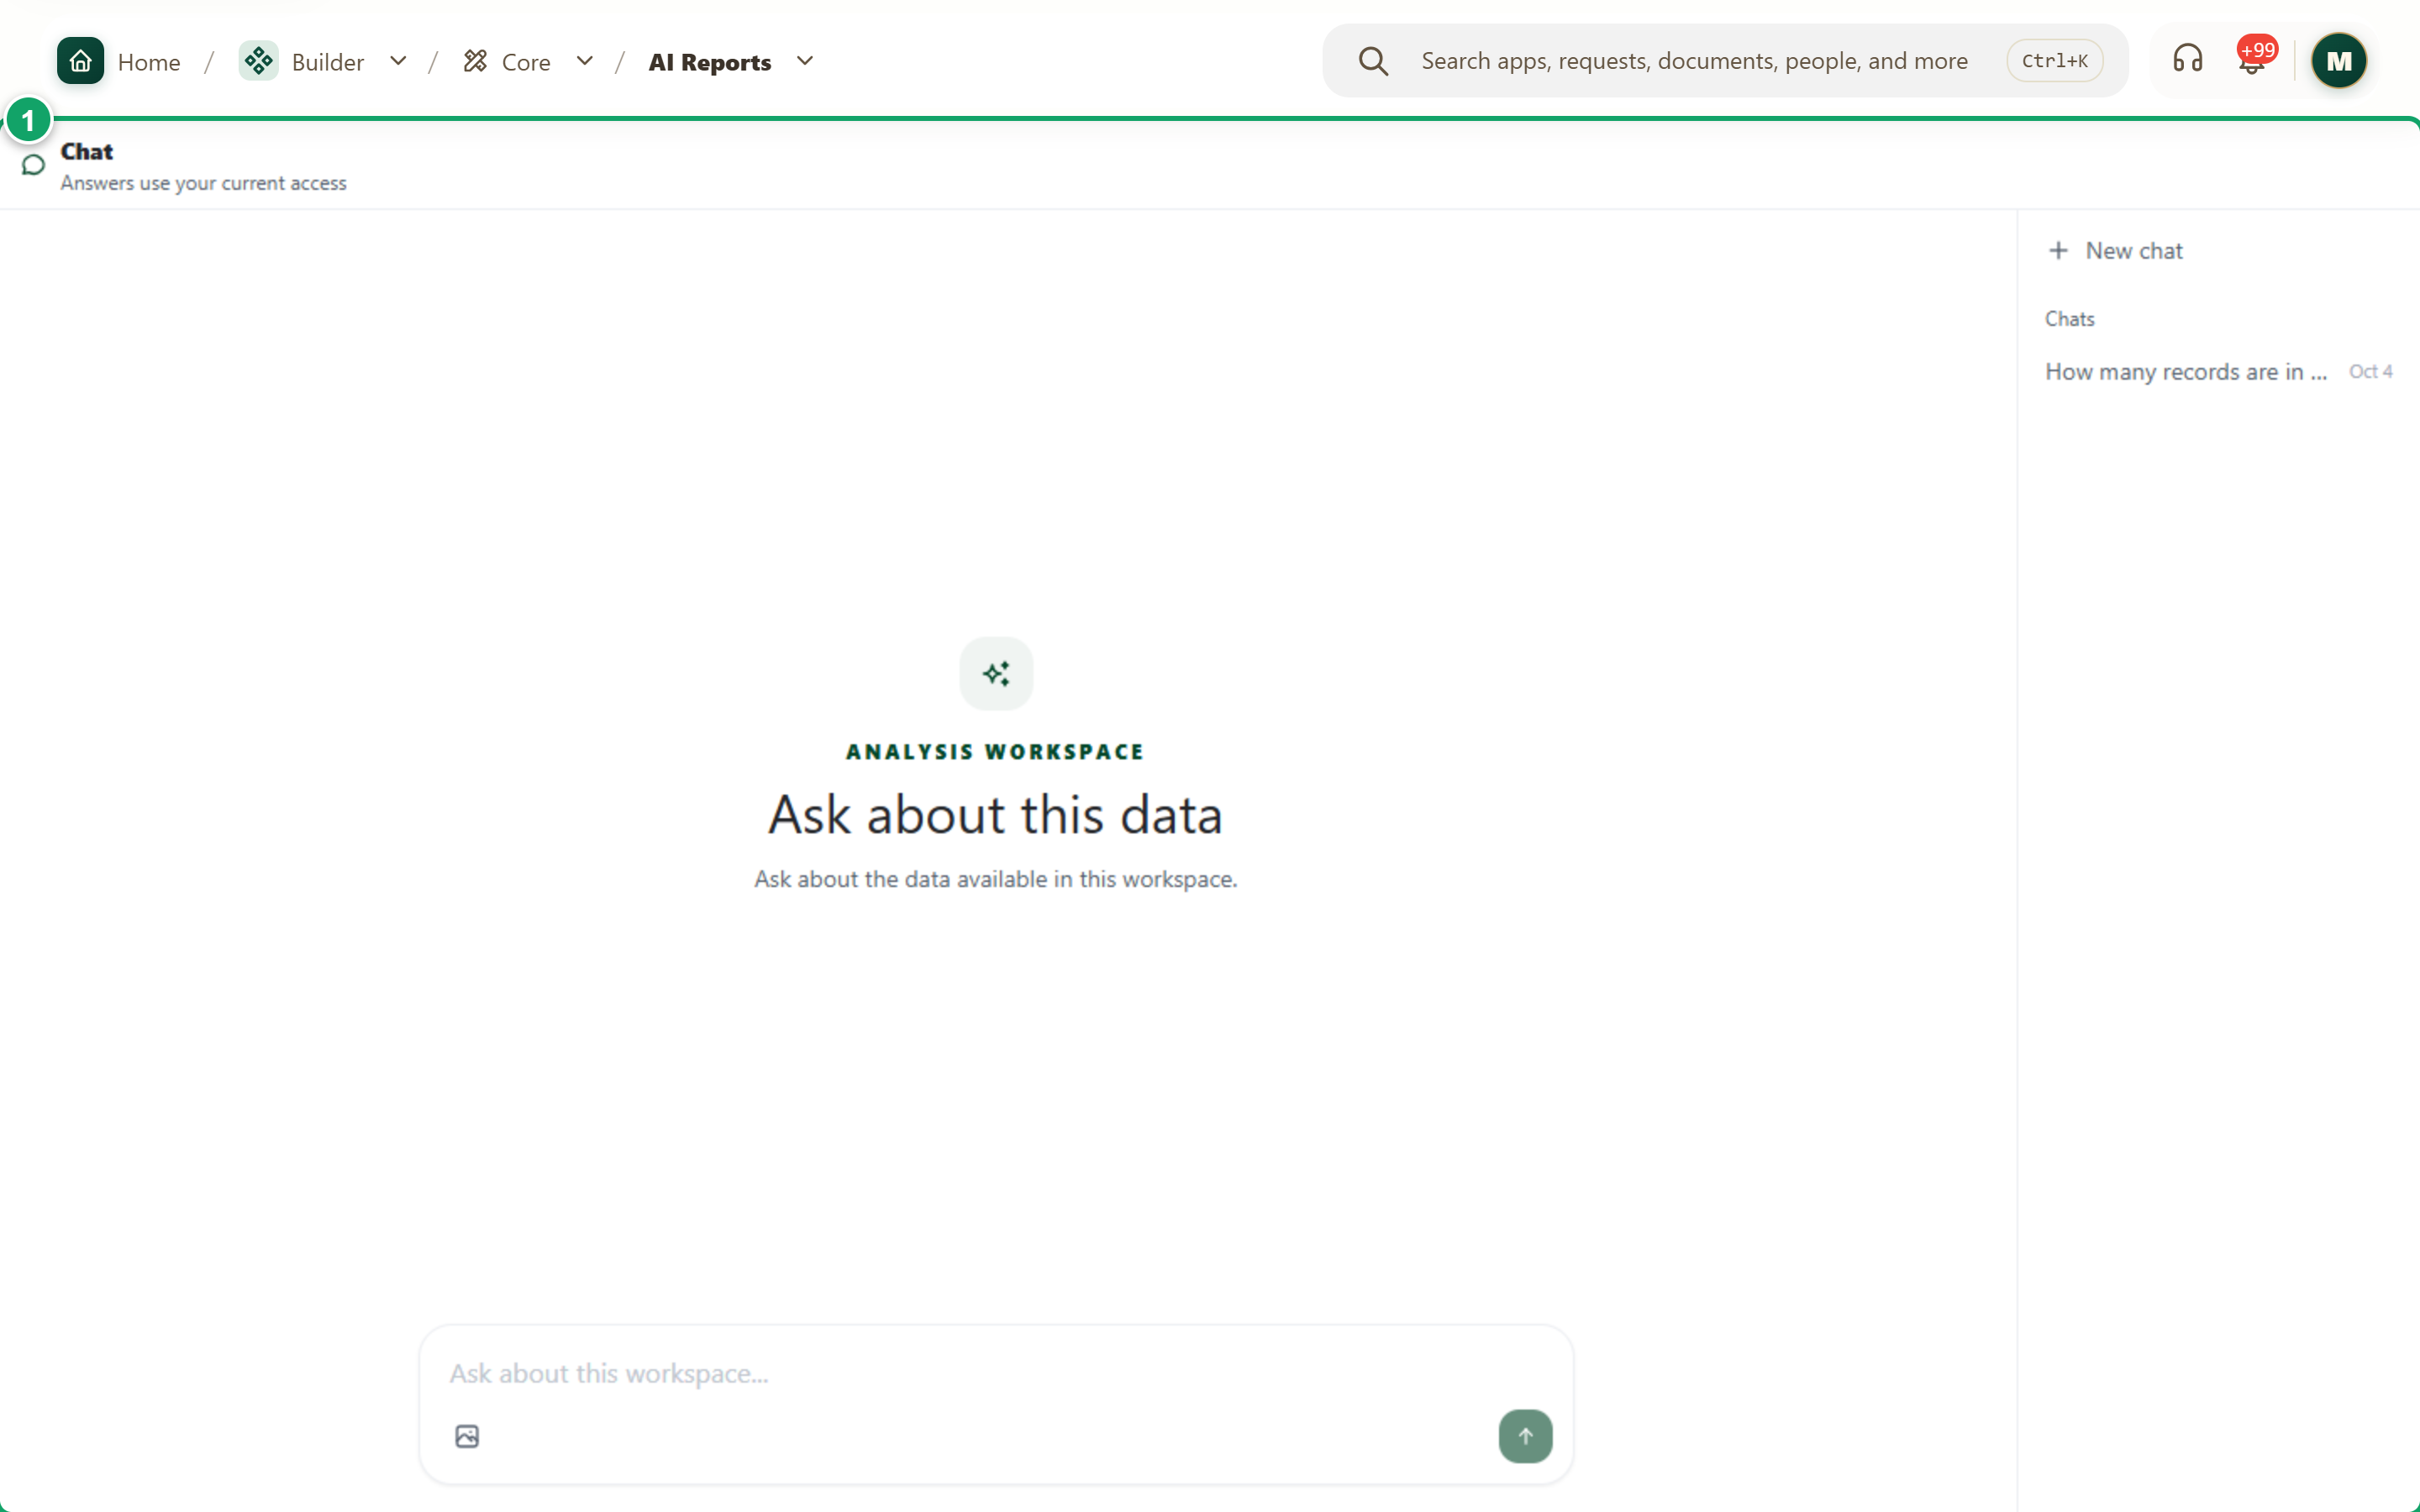
\includegraphics[width=0.95\linewidth,height=0.72\textheight,keepaspectratio]{figures/screens/ch06-ai-reports-en.png}
\caption{The “AI Reports” workspace}
\label{fig:builder-ai-reports-screen}
\shotnote{The same analytics workspace opens in chat mode. ① The chat area: where you write your question and read the report.}
\end{figure}


\begin{table}[H]
\centering
\caption{When to use reports and when to use dashboards}
\label{tab:builder-ai-reports-data}
\begin{tabularx}{\linewidth}{R{3.6cm} Y}
\rcHeaderRow
\thh{Need} & \thh{Best fit}\\
A one-off question & “AI Reports”: ask and read the answer.\\
Recurring follow-up & “AI Dashboards” or “Dashboards”, because a dashboard is refreshed and reviewed regularly.\\
Sharing with the team & Publish the dashboard from “Pages”; chat answers do not appear in navigation.\\
\end{tabularx}
\end{table}

\begin{figure}[H]
\centering
\begin{tikzpicture}[node distance=0.5cm]
\node[stepBox] (a) {A clear question with a period};
\node[stepBox,below=of a] (b) {Read the report};
\node[stepBox,below=of b] (c) {Check one known number};
\draw[flowsTo] (a) -- (b);
\draw[flowsTo] (b) -- (c);
\end{tikzpicture}
\rclegend
\caption{Asking a question and checking the answer}
\label{fig:builder-ai-reports-flow}
\shotnote{The diagram ends with a check, because the answer is built on the data the person asking can read and on how the AI understood the question. If one number you know matches the report, you can trust the rest of the answer more.}
\end{figure}

\subsection{Steps and check}
\begin{enumerate}
\item Open “AI Reports” and wait for the chat to load.
\item Write your question with the time period and the record type you mean.
\item Read the report, and compare one number in it with what you know before relying on it.
\end{enumerate}

\textbf{Check and recovery:} an answer referring to your organization's data should arrive. If the page does not open, review your seat and permissions as for “AI Dashboards”. If the answer looks incomplete, rephrase the question with the record type and period.
